% !TEX program = pdflatex
% ---------------------------------------------------------------
%  Artículo: selección de streamlines con pesos SIFT2, LiFE y COMMIT
%  CIMAT, Unidad Aguascalientes
%  Compilar con:  pdflatex articulo_tractografia.tex  (dos veces)
%  Logo: coloca el archivo  logo_cimat.png  (o .jpg / .pdf) en la
%  misma carpeta; si no existe, se dibuja un recuadro de aviso.
% ---------------------------------------------------------------
\documentclass[11pt,a4paper]{article}

\usepackage[utf8]{inputenc}
\usepackage[T1]{fontenc}
\usepackage{mathptmx}
\usepackage[scaled=.90]{helvet}
\renewcommand{\ttdefault}{pcr}
% Idioma: babel en español si está instalado; si no, rótulos manuales.
\IfFileExists{spanish.ldf}{%
  \usepackage[spanish,es-tabla,es-noshorthands]{babel}%
  \decimalpoint
}{%
  \AtBeginDocument{%
    \renewcommand{\figurename}{Figura}\renewcommand{\tablename}{Tabla}%
    \renewcommand{\refname}{Referencias}\renewcommand{\appendixname}{Ap\'endice}}%
}
\usepackage[top=2.6cm,bottom=2.4cm,left=2.4cm,right=2.4cm,headheight=15pt]{geometry}
\usepackage{microtype}
\usepackage{amsmath,amssymb}
\usepackage{booktabs,tabularx,array,multirow}
\usepackage{graphicx}
\usepackage{xcolor}
\usepackage{caption}
\usepackage{enumitem}
\usepackage{fancyhdr}
\usepackage{float}
\usepackage{tikz}
\usetikzlibrary{arrows.meta,positioning,shapes.geometric,fit,calc}
\usepackage{pgfplots}
\pgfplotsset{compat=1.16}
\usepackage[colorlinks=true,linkcolor=cimatblue,citecolor=cimatblue,urlcolor=cimatblue]{hyperref}

% ----- colores (azul institucional sobrio) -----
\definecolor{cimatblue}{RGB}{0,62,126}
\definecolor{cimatgray}{RGB}{90,90,90}
\definecolor{boxfill}{RGB}{232,240,250}
\definecolor{okgreen}{RGB}{46,125,50}
\definecolor{warnorange}{RGB}{239,108,0}

% ----- formato -----
\setlength{\parindent}{0pt}
\setlength{\parskip}{0.55em}
\renewcommand{\arraystretch}{1.12}
\captionsetup{font=small,labelfont={bf,color=cimatblue},labelsep=period,margin=0.5cm}
\setlist{itemsep=0.15em,topsep=0.3em}

\pagestyle{fancy}
\fancyhf{}
\renewcommand{\headrulewidth}{0.4pt}
\fancyhead[L]{\small\color{cimatgray}Selección de streamlines con pesos SIFT2, LiFE y COMMIT}
\fancyhead[R]{\small\color{cimatgray}CIMAT, Unidad Aguascalientes}
\fancyfoot[C]{\small\thepage}

\usepackage{titlesec}
\titleformat{\section}{\large\bfseries\color{cimatblue}}{\thesection.}{0.6em}{}
\titleformat{\subsection}{\normalsize\bfseries\color{cimatblue}}{\thesubsection}{0.6em}{}
\titlespacing*{\section}{0pt}{1.4em}{0.5em}
\titlespacing*{\subsection}{0pt}{1.0em}{0.35em}

\newcommand{\code}[1]{\texttt{\small #1}}
\newcommand{\eps}{\varepsilon}

% ----- logo -----
\newcommand{\cimatlogo}{%
  \IfFileExists{logoCimat.png}{
\includegraphics[height=2cm]{logoCimat.png}}{%
  \IfFileExists{logoCimat.jpg}{
\includegraphics[height=2cm]{logoCimat.png}}{%
  \IfFileExists{logoCimat.pdf}{\includegraphics[height=2cm]{logo_cimat.pdf}}{%
  \fbox{\parbox[c][2.2cm][c]{3.6cm}{\centering\footnotesize\color{cimatgray}%
  Coloca aqu\'i el logo\\[2pt]\texttt{logoCimat.png}}}}}}}

\begin{document}

% =================== ENCABEZADO INSTITUCIONAL ===================
\thispagestyle{empty}
\noindent
\begin{minipage}[c]{0.28\textwidth}
  \cimatlogo
\end{minipage}%
\hfill
\begin{minipage}[c]{0.68\textwidth}
  \raggedleft
  {\large\bfseries\color{cimatblue} Centro de Investigaci\'on en Matem\'aticas, A.C.}\\[2pt]
  {\color{cimatgray} Unidad Aguascalientes}\\[2pt]
  {\small\color{cimatgray} Maestr\'ia en Modelaci\'on y Optimizaci\'on de Procesos}
\end{minipage}

\vspace{0.3em}
{\color{cimatblue}\rule{\textwidth}{1.2pt}}

\vspace{1.2em}
\begin{center}
  {\LARGE\bfseries\color{cimatblue}
  Selecci\'on de \textit{streamlines} en tractograf\'ia mediante pesos SIFT2, LiFE y COMMIT:
  normalizaci\'on, filtrado y evaluaci\'on contra el \textit{ground truth}
  del fantoma ISMRM\par}
  \vspace{1.0em}
 \begin{tabular}{ccc}
  {\large Sarai Hernandez } & {\large Andrea Martinez } & {\large Jaqueline Barrajas }\\
  {\large Mario }           & {\large Max }    & {\large Ricardo}\\
  {\large Pablo}
\end{tabular}\par
  % Para agregar coautores:  {\large Sarai Hernandez Montes, Nombre Apellido, \dots\par}
  \vspace{0.3em}
  {\small\color{cimatgray}
  CIMAT, Unidad Aguascalientes\\
  Laboratorio de Resoluci\'on de Problemas~I\\
  Noviembre de 2026 \,---\, trabajo en progreso\par}
\end{center}

\vspace{0.6em}
\begin{center}
\begin{minipage}{0.9\textwidth}
\small
\textbf{Resumen.}\;
Los algoritmos de tractograf\'ia producen conjuntos de \textit{streamlines} con una
proporci\'on alta de trayectorias que no corresponden a ning\'un haz real. SIFT2, LiFE y
COMMIT asignan un peso a cada \textit{streamline} a partir de la se\~nal de difusi\'on y
pueden usarse para descartar los que no se sostienen con ella. Sobre el fantoma del
desaf\'io ISMRM generamos, con MRtrix3, un tractograma de 100\,000 \textit{streamlines} el cual obtuvo tres vectores de pesos (m\'as COMMIT2 como variante) y los comparamos con
el \textit{ground truth} (GT) de 189\,985 \textit{streamlines} y 21 haces, a nivel de
matriz de conectividad $84\times 84$ e hilo por hilo. LiFE es el \'unico m\'etodo cuya
matriz mejora al simple conteo de hilos (90.7\,\% del peso en conexiones reales contra
80.5\,\%). Hilo por hilo, los pesos de COMMIT y SIFT2 ordenan al rev\'es de lo esperado
(AUC 0.42 y 0.35), mientras que COMMIT2 y LiFE s\'i separan hilos buenos de malos
(0.68 y 0.66); la longitud del hilo, por s\'i sola, alcanza 0.75. La mejor combinaci\'on
(COMMIT2 + LiFE) baja la proporci\'on de hilos falsos de 45.2\,\% a 33.8\,\% conservando
los 21 haces. Adem\'as, describimos una poda espacial que reduce el c\'alculo de la
distancia de Hausdorff contra el GT de $\approx 22 s$ a $\approx 0.12 s$ por hilo sin cambiar
el resultado. El entrenamiento de un modelo que combine los tres pesos queda como
trabajo pendiente.

\medskip
\textbf{Palabras clave:} tractograf\'ia, \textit{streamlines}, SIFT2, LiFE, COMMIT,
distancia de Hausdorff, conectividad estructural.
\end{minipage}
\end{center}

\vspace{0.4em}
{\color{cimatblue}\rule{\textwidth}{0.6pt}}

% Pendientes,
% - el tiempo de que se tardo en ejecutar
% - el tiempo de cómputo 
% parfor en python
% - estimaciones de tiempo 

% =================== 1. INTRODUCCIÓN ===================
\section{Introducci\'on}

La tractograf\'ia de resonancia magn\'etica de difusi\'on (dMRI) reconstruye las v\'ias de
materia blanca siguiendo, v\'oxel a v\'oxel, las direcciones locales de las fibras. El
resultado es un conjunto de curvas 3D llamadas \textit{streamlines} (también llamadas ``hilos'').
Como el algoritmo solo conoce la direcci\'on local y no verifica que el recorrido completo
exista, una parte importante de los hilos es plausible pero falsa. Esto se constat\'o en el desaf\'io ISMRM de tractograf\'ia \cite{maierhein2017}, en el que algunos métodos detectaron la mayor\'ia de los haces reales y, al mismo tiempo, muchos m\'as haces
inv\'alidos que v\'alidos. Su fantoma simulado, con los haces reales conocidos
de antemano, es el conjunto de datos de este trabajo y la referencia contra la
que se mide todo lo que se va a ver.

Métodos como SIFT2 \cite{smith2015}, LiFE \cite{pestilli2014} y COMMIT \cite{daducci2015}
atacan el problema volviendo a los datos de difusi\'on que originaron el
tractograma. Dado un tractograma fijo, estiman qu\'e contribuci\'on de cada hilo
hace falta para reproducir lo que se midi\'o, ya sea sobre la se\~nal misma
(LiFE y COMMIT) o sobre la FOD estimada a partir de ella (SIFT2). Los tres
devuelven un peso por hilo, pero en escalas y con significados distintos, por lo
que no es evidente c\'omo compararlos, combinarlos ni usarlos para decidir qu\'e
hilos conservar.

%Métodos como el  SIFT2 \cite{smith2015}, LiFE \cite{pestilli2014} y COMMIT \cite{daducci2015} atacan el problema desde la se\~nal. Dado un tractograma fijo, estiman cu\'anto necesita cada hilo para explicar la imagen de difusi\'on medida. Los tres devuelven un peso por hilo, pero en escalas y con significados distintos, por lo que no es evidente c\'omo compararlos, combinarlos ni usarlos para decidir qu\'e hilos conservar.

Este trabajo documenta un procedimiento reproducible que parte de un \'unico
tractograma, obtiene los tres vectores de pesos y los eval\'ua contra el GT. 

El objetivo de este trabajo consiste en los siguientes pasos:

\begin{enumerate}[label=\textbf{\Alph*.}]
  \item Obtener un vector de 100\,000 pesos por m\'etodo ($x_S$, $x_L$, $x_C$).
  \item Normalizar cada vector a $(0,1)$ y descartar los hilos con peso menor que un umbral $\eps$, m\'etodo por m\'etodo.
  \item Etiquetar cada hilo como correspondiente o no al GT mediante la distancia de Hausdorff;
  \item Entrenar un modelo $(x_S,x_L,x_C)\mapsto\{0,1\}$ con esa etiqueta y comparar el tractograma filtrado por el modelo con el GT.
\end{enumerate}

El trabajo se complement\'o con matrices de conectividad, con COMMIT2 y el barrido de su par\'ametro de regularizaci\'on $\lambda$, y con una normalizaci\'on por percentiles.

%Los pasos A y B (parcial) est\'an completos; el C est\'a listo para ejecutarse y el D est\'a pendiente (secci\'on~\ref{sec:estado}). Adem\'as del objetivo, se hizo trabajo complementario: matrices de conectividad, COMMIT2 y su barrido de regularizaci\'on, y un normalizaci\'on por percentiles.

% NOTA: Falta agregar el contenido del reporte

\textbf{Contribuciones.} (i) Un pipeline de extremo a extremo con un tractograma
compartido por todos los m\'etodos (verificado por \textit{checksum}); (ii) una comparaci\'on
de los cuatro m\'etodos a nivel de conexi\'on y de hilo, con m\'etricas invariantes a la
escala; (iii) la identificaci\'on de un fuerte sesgo por longitud, tanto en los pesos como
en la etiqueta de evaluaci\'on; y (iv) un c\'alculo de la etiqueta de Hausdorff con poda
espacial, verificado contra fuerza bruta.

% =================== 2. Marco Teórico ===================

\section{Marco Teórico}

% ===================  DATOS ===================
\subsection{Presentación de los datos}

Se usa el fantoma del desaf\'io ISMRM (archivos \code{ISMRM\_2023\_b3000}). La
Tabla~\ref{tab:datos} resume las entradas.

\begin{table}[H]
\centering
\small
\begin{tabularx}{\textwidth}{@{}lX@{}}
\toprule
\textbf{Elemento} & \textbf{Descripci\'on}\\
\midrule
Imagen de difusi\'on & 65 mediciones por v\'oxel: 1 imagen $b=0$ y 64 direcciones con $b=3000$ s/mm$^2$.\\
Parcelaci\'on & 84 regiones (\code{Parcels\_free.nii}); la regi\'on 15 no existe en la imagen, por lo que su fila y columna quedan en cero.\\
\textit{Ground truth} (GT) & 189\,985 \textit{streamlines} agrupados en 21 haces; su matriz de conectividad tiene 529 conexiones reales de los 3\,486 pares posibles.\\
Tractograma de trabajo & 100\,000 hilos (\code{tracks\_100k.tck}), longitud media 92.13~mm y mediana 95.21~mm; \textit{checksum} MD5 \code{66ba3e6e\dots}. Todos los m\'etodos pesan estos mismos hilos, en este orden.\\
\bottomrule
\end{tabularx}
\caption{Datos de entrada y tractograma de trabajo.}
\label{tab:datos}
\end{table}

Los 100\,000 hilos no son ``todos los posibles'': \code{tckgen -select 100000} se detiene al
aceptar ese n\'umero, que es un tama\~no elegido. Que los tres m\'etodos pesen exactamente
los mismos hilos es lo que permite compararlos hilo por hilo.

% =================== 3. METODOLOGÍA ===================
\section{Metodolog\'ia}

En la Figura~\ref{fig:flujo} se muestra el flujo completo (v\'ease Ap\'endice~\ref{app:repro} para los comandos exactos, paso por paso).

\begin{figure}[H]
\centering
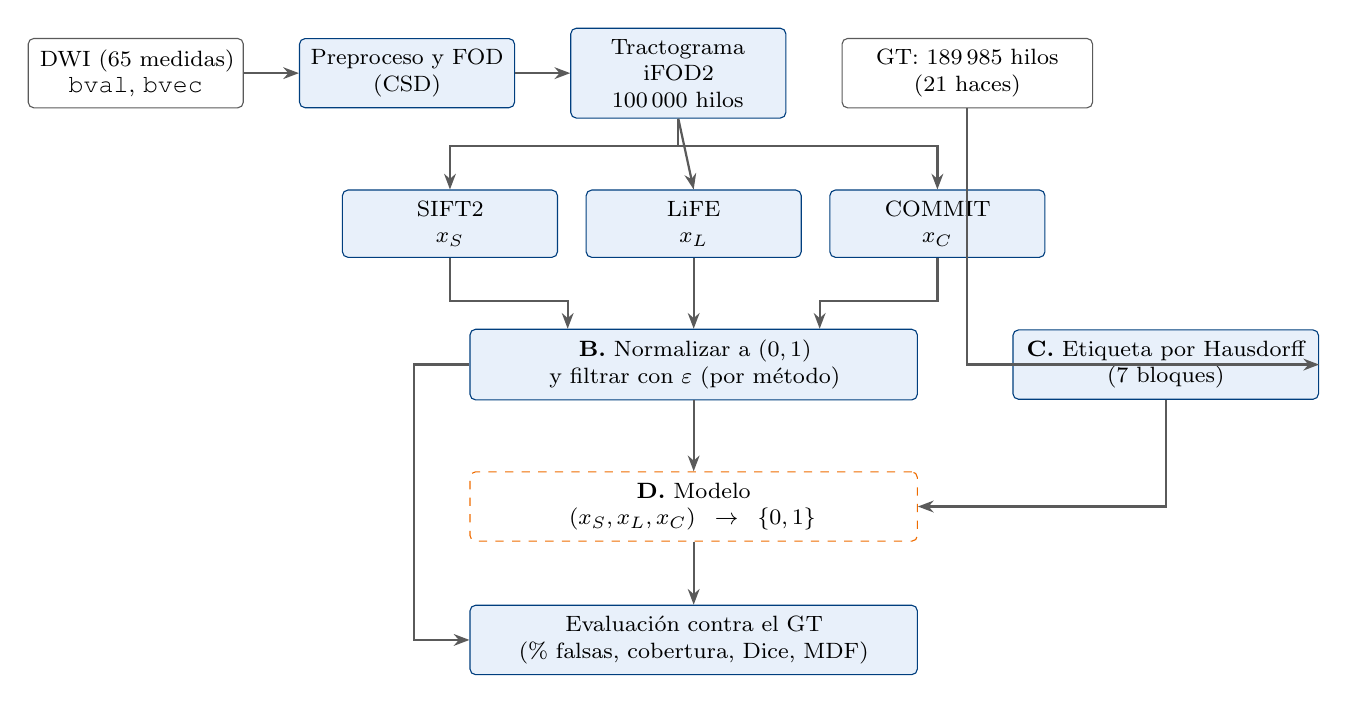
\begin{tikzpicture}[
  font=\footnotesize,
  node distance=0.55cm and 0.7cm,
  box/.style={draw=cimatblue,fill=boxfill,rounded corners=2pt,align=center,
              minimum height=0.85cm,inner sep=4pt,text width=2.45cm},
  wide/.style={box,text width=5.4cm},
  data/.style={draw=cimatgray,fill=white,rounded corners=2pt,align=center,
               minimum height=0.85cm,inner sep=4pt,text width=2.45cm},
  todo/.style={box,fill=white,dashed,draw=warnorange},
  arr/.style={-{Stealth[length=2mm]},thick,color=cimatgray}
]
% fila 1
\node[data] (dwi) {DWI (65 medidas)\\ \code{bval}, \code{bvec}};
\node[box,right=of dwi] (fod) {Preproceso y FOD\\ (CSD)};
\node[box,right=of fod] (tck) {Tractograma iFOD2\\ 100\,000 hilos};
\node[data,right=of tck,text width=2.9cm] (gt) {GT: 189\,985 hilos\\ (21 haces)};
% fila 2: métodos
\node[box,below=0.9cm of tck,xshift=-2.9cm] (sift) {SIFT2\\ $x_S$};
\node[box,right=0.35cm of sift] (life) {LiFE\\ $x_L$};
\node[box,right=0.35cm of life] (commit) {COMMIT\\ $x_C$};
% fila 3
\node[wide,below=0.9cm of life] (norm) {\textbf{B.} Normalizar a $(0,1)$\\ y filtrar con $\eps$ (por m\'etodo)};
\node[box,right=1.2cm of norm,text width=3.6cm] (haus) {\textbf{C.} Etiqueta por Hausdorff\\ (7 bloques)};
% fila 4
\node[todo,below=0.9cm of norm,text width=5.4cm] (mod) {\textbf{D.} Modelo\\ $(x_S,x_L,x_C)\to\{0,1\}$};
% fila 5
\node[wide,below=0.8cm of mod] (eval) {Evaluaci\'on contra el GT\\ (\% falsas, cobertura, Dice, MDF)};

\draw[arr] (dwi) -- (fod);
\draw[arr] (fod) -- (tck);
\draw[arr] (tck.south) -- ++(0,-0.35) -| (sift.north);
\draw[arr] (tck.south) -- ++(0,-0.35) -| (commit.north);
\draw[arr] (tck.south) -- (life.north);
\draw[arr] (sift.south) |- ($(norm.north)+(-1.6,0.35)$) -- ($(norm.north)+(-1.6,0)$);
\draw[arr] (life.south) -- (norm.north);
\draw[arr] (commit.south) |- ($(norm.north)+(1.6,0.35)$) -- ($(norm.north)+(1.6,0)$);
\draw[arr] (gt.south) |- (haus.east);
\draw[arr] (norm.south) -- (mod.north);
\draw[arr] (haus.south) |- (mod.east);
\draw[arr] (mod.south) -- (eval.north);
\draw[arr] (norm.west) -- ++(-0.7,0) |- (eval.west);
\end{tikzpicture}
\caption{Flujo del proyecto. Las cajas con borde punteado est\'an pendientes. El tractograma es el archivo central que comparten los tres m\'etodos y la etiqueta.}
\label{fig:flujo}
\end{figure}

\subsection{Preprocesamiento y tractograf\'ia}

Con MRtrix3 \cite{tournier2019} se estima la m\'ascara cerebral (\code{dwi2mask}), la
respuesta de fibra \'unica (\code{dwi2response tournier}) y la funci\'on de distribuci\'on de
orientaciones de fibra (FOD) por deconvoluci\'on esf\'erica restringida
(\code{dwi2fod csd}, \cite{tournier2007}). El tractograma se genera con el algoritmo
probabil\'istico iFOD2 \cite{tournier2010} (\code{tckgen}), sembrando dentro de la m\'ascara
y deteni\'endose al aceptar 100\,000 hilos.

\textbf{Correcci\'on del eje $y$}. Con el archivo \code{bvec} sin modificar, las
direcciones del gradiente resultan incoherentes con el GT; por lo que se optó por invertir el signo de la
componente $y$ para corregirlo. El efecto sobre la tractograf\'ia es grande (longitud media de
$\approx$36--42~mm a $\approx$92~mm). En cambio, los pesos de SIFT2 casi no cambian
(correlaci\'on 0.989). En COMMIT y LiFE no se aisl\'o su efecto, as\'i que no puede
atribuirse a esta correcci\'on una parte concreta de las mejoras observadas.

\subsection{Pesos por hilo}

A continuación se describen los cuatro m\'etodos que asignan un peso a cada hilo del tractograma. Todos devuelven 100\,000 pesos no negativos en el orden de \code{tracks\_100k.tck}, pero en escalas y con significados distintos.

\begin{itemize}
    \item \textbf{SIFT2} \cite{smith2015} (\code{tcksift2}) 
\end{itemize}

Este método ajusta un factor multiplicativo por hilo, cercano a 1, de modo que la densidad de fibra del tractograma coincida con la de la FOD;
sus pesos nunca son cero.

\begin{itemize}
    \item \textbf{LiFE} \cite{pestilli2014} (DIPY \cite{garyfallidis2014}, \code{FiberModel}) 
\end{itemize}

El método ajusta por m\'inimos cuadrados no negativos un coeficiente $\beta\ge 0$ por hilo sobre la se\~nal. El archivo de afinidad (\textit{affine}) debe pasarse invertido a DIPY.

\begin{itemize}
    \item \textbf{COMMIT} \cite{daducci2015} 
\end{itemize}

El método modela la se\~nal como la suma de la contribuci\'on de cada hilo (compartimento intra-axonal, \textit{Stick}), el agua alrededor de los axones (\textit{Zeppelin}) y el agua libre (\textit{Ball}) \cite{panagiotaki2012}. Con $A$ el
diccionario de se\~nales y $y$ la se\~nal medida, resuelve
\begin{equation}\label{eq:commit}
  \min_{x\ge 0}\; \lVert A x - y\rVert_2^2 ,
\end{equation}
donde las primeras 100\,000 entradas de $x$ son los pesos de los hilos. Se us\'o el modelo
Stick--Zeppelin--Ball con $d_\parallel=1.7\times10^{-3}$, $d_{\perp}^{\mathrm{zep}}=0.51\times10^{-3}$
y $d_{\mathrm{iso}}\in\{1.7,3.0\}\times10^{-3}$~mm$^2$/s, hasta tres picos por v\'oxel
(\code{sh2peaks}) y AMICO \cite{daducci2015amico} para ajustar. COMMIT no usa el GT ni
inventa hilos: solo elige entre los que se le dan. Como su peso es por unidad de longitud,
un hilo largo necesita menos peso para aportar la misma se\~nal, y los cortos quedan
favorecidos.

Por otro lado, \textbf{COMMIT2} \cite{schiavi2020} parte del mismo ajuste (ir a la ecuación~\eqref{eq:commit}) y le añade una penalizaci\'on por grupos. Los hilos que
unen el mismo par de regiones forman un grupo y el ajuste prefiere apagar conexiones
completas poco respaldadas por la se\~nal. El par\'ametro $\lambda$ controla la intensidad.

\subsection{Matriz de conectividad}

La matriz de conectividad describe c\'omo se conectan entre s\'i las 84 regiones en que se
divide el cerebro. Se construye con \code{tck2connectome} (\code{-symmetric
-zero\_diagonal}), y la celda $(i,j)$ acumula lo que aporta cada hilo cuyos extremos caen
en las regiones $i$ y $j$. Esa condici\'on deja fuera al 27\,\% de los hilos, que no
alcanza ninguna regi\'on y no entra en ninguna matriz. Al compartir tractograma, todos los
m\'etodos pierden los mismos hilos.

Lo \'unico que cambia entre variantes es cu\'anto aporta cada hilo a su celda. En el \textbf{conteo} aporta 1. En las matrices ponderadas aporta su peso. En la matriz de COMMIT ponderada por longitud, cada hilo aporta el producto de su peso y su longitud, de modo que, el peso de COMMIT esté definido por unidad de longitud.

%Con \code{tck2connectome}, la celda $(i,j)$ suma los pesos de los hilos cuyos dos extremos caen en las regiones $i$ y $j$ (opciones \code{-symmetric -zero\_diagonal}). Con peso 1 para todos los hilos se obtiene el \textbf{conteo}, que act\'ua como control: si un m\'etodo no supera al conteo, sus pesos no aportan informaci\'on a nivel de matriz. Una variante, ``COMMIT $\times$ longitud'', multiplica cada peso por la longitud del hilo para quitar el sesgo hacia los cortos. El 27\,\% de los hilos no termina en ninguna regi\'on y queda fuera de toda matriz, igual para los tres m\'etodos.

\subsection{Normalizaci\'on y filtrado}
\label{sec:norm}

Cada m\'etodo usa otra escala (COMMIT $\sim10^{-3}$, SIFT2 $\sim1$, LiFE de decenas), por
lo que los pesos crudos no se pueden promediar. Se consideran dos normalizaciones:
\begin{itemize}
  \item \textbf{Por el m\'aximo}: $\tilde w_i = w_i/\max_k w_k\in[0,1]$.
        El hilo es v\'alido si $\tilde w_i\ge\eps$.
  \item \textbf{Por percentil}: los hilos con $w=0$ se quedan en 0 y
        los de $w>0$ reciben su rango dividido entre $n$ (rango promedio en empates).
        Los percentiles de varios m\'etodos se promedian y se filtra con un umbral $u$.
        Se prob\'o adem\'as una variante que calcula el percentil dentro de 10 rangos de longitud.
\end{itemize}

\subsection{Etiqueta por hilo}

\textbf{Hausdorff.} Para un hilo $y$ del tractograma y un hilo $g$ del GT,
\begin{equation}
  d_H(y,g)=\max\Big\{\max_{p\in y} d(p,g),\; \max_{q\in g} d(q,y)\Big\},
\end{equation}
y $y$ ``corresponde al GT'' si $\min_g d_H(y,g)<\eps_H$. La versi\'on dirigida
(primer t\'ermino) responde a ``\textquestiondown este hilo est\'a dentro de un haz real?''.
Calcularla contra los 189\,985 hilos del GT es costoso (Secci\'on~\ref{sec:haus}).

\textbf{MDF.} La distancia media directa con volteo (\textit{minimum average direct-flip})
\cite{garyfallidis2012} remuestrea ambos hilos a $K=20$ puntos:
\begin{equation}
  \mathrm{MDF}(s,t)=\min\Big\{\tfrac1K\sum_{i=1}^{K}\lVert s_i-t_i\rVert,\;
                       \tfrac1K\sum_{i=1}^{K}\lVert s_i-t_{K+1-i}\rVert\Big\}.
\end{equation}

Un hilo es \textit{verdadero} si su MDF m\'inima a hilos representativos de alg\'un haz del GT es menor que 5~mm; si no, es \textit{falso}. Es mucho m\'as barata ($\approx$2~min para los 100\,000 hilos), y es la etiqueta con que se obtuvieron los resultados de la Secci\'on~\ref{sec:resultados} mientras se calcula la de Hausdorff.

\subsection{M\'etricas}

\textbf{Por conexi\'on} (matriz contra el GT): n\'umero de conexiones con peso positivo;
cu\'antas de las 529 reales sobreviven; \% del peso total que cae en conexiones reales;
AUC por conexi\'on; y correlaci\'on de Pearson con la matriz del GT. Todas son invariantes
a la escala de los pesos.

\textbf{Por hilo:} AUC del peso como puntaje para predecir la etiqueta (0.5 = azar).

\textbf{Del tractograma filtrado} (hilo asignado al haz de menor MDF si $<5$~mm; las
m\'etricas de v\'oxel se calculan contra la m\'ascara del haz verdadero, con VP, FP y FN):
haces detectados (de 21); \% de fibras falsas $=$ hilos sin haz / total;
cobertura $=\mathrm{VP}/(\mathrm{VP}+\mathrm{FN})$; desborde $=\mathrm{FP}/(\mathrm{VP}+\mathrm{FN})$;
Dice $=2\mathrm{VP}/(2\mathrm{VP}+\mathrm{FP}+\mathrm{FN})$; y MDF sim\'etrico (mm).

% Faltan los métodos de aprendizaje 


% =================== 4. RESULTADOS ===================
\section{Resultados}
\label{sec:resultados}

\subsection{Pesos, escalas y filtrado simple}

Los pesos no son comparables en valor absoluto. COMMIT pone en cero 44\,780 hilos (44.8\,\%; NRMSE del ajuste $0.106\pm0.039$), LiFE 25\,388 (25.4\,\%) y SIFT2 ninguno. Con la normalizaci\'on por el m\'aximo y $\eps=0.1$, SIFT2 conserva 93\,978 hilos (94.0\,\%) y LiFE 50\,239 (50.2\,\%); con $\eps=0.01$ conservan 100\,\% y 72\,\%, respectivamente. Es decir, $\eps=0.01$ no filtra nada en SIFT2, porque sus pesos se concentran alrededor de 1. Por eso el umbral conviene barrerlo en lugar de fijarlo, y comparar m\'etodos con el mismo
n\'umero de hilos conservados.

\subsection{Nivel de conexi\'on}

\begin{table}[H]
\centering
\small
\begin{tabularx}{\textwidth}{@{}Xrrrrr@{}}
\toprule
\textbf{Matriz} & \textbf{Conex.\,$>0$} & \textbf{Del GT} & \textbf{\% peso en GT} & \textbf{AUC} & \textbf{Pearson}\\
\midrule
Conteo (sin pesos)         & 1\,322 & 460 & 80.5 & 0.857 & 0.894\\
SIFT2                      & 1\,322 & 460 & 74.6 & 0.850 & 0.795\\
COMMIT                     & 1\,203 & 446 & 63.8 & 0.829 & 0.731\\
COMMIT $\times$ longitud   & 1\,203 & 446 & 79.0 & 0.846 & 0.881\\
COMMIT2 ($\lambda=10^{-2}$)& 86     & 70  & 91.9 & 0.564 & 0.788\\
\textbf{LiFE}              & 1\,168 & 442 & \textbf{90.7} & 0.851 & \textbf{0.923}\\
\bottomrule
\end{tabularx}
\caption{Matrices $84\times84$ contra el GT (529 conexiones reales de 3\,486 pares). La
fila ``conteo'' es el control.}
\label{tab:matrices}
\end{table}

LiFE es el \'unico cuya matriz queda por encima del conteo en \% del peso en el GT (90.7
contra 80.5) y en Pearson (0.923 contra 0.894); descarta 154 de las 1\,322 conexiones y
pierde solo 18 reales. COMMIT y SIFT2 quedan por debajo del conteo, y COMMIT solo se
acerca al multiplicar por la longitud (Pearson de 0.731 a 0.881). Con $\lambda=10^{-2}$,
COMMIT2 deja \'unicamente 86 conexiones: limpia mucho pero apaga conexiones reales.

\subsection{Nivel de hilo}

\begin{figure}[H]
\centering
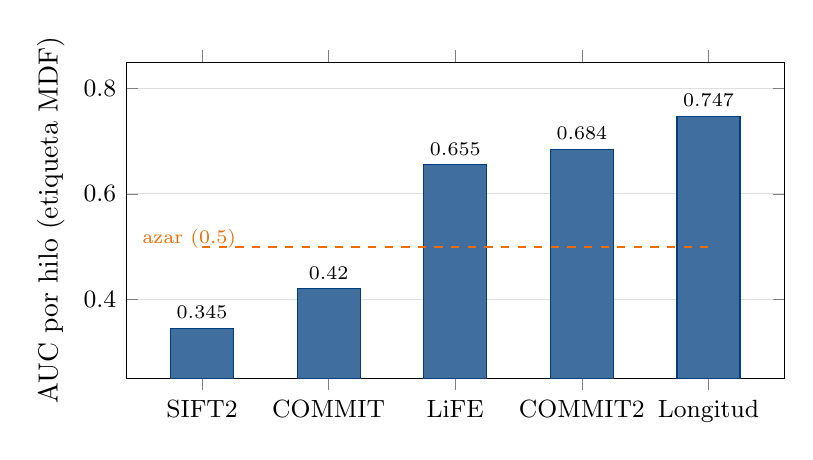
\begin{tikzpicture}
\begin{axis}[
  ybar, bar width=0.8cm, width=0.82\textwidth, height=5.6cm,
  ymin=0.25, ymax=0.85, ylabel={AUC por hilo (etiqueta MDF)},
  symbolic x coords={SIFT2,COMMIT,LiFE,COMMIT2,Longitud},
  xtick=data, nodes near coords, nodes near coords style={font=\scriptsize},
  every node near coord/.append style={/pgf/number format/fixed,/pgf/number format/precision=3},
  ymajorgrids, grid style={gray!25}, tick label style={font=\small},
  enlarge x limits=0.15
]
\addplot[fill=cimatblue!75,draw=cimatblue] coordinates {(SIFT2,0.345) (COMMIT,0.420) (LiFE,0.655) (COMMIT2,0.684) (Longitud,0.747)};
\draw[dashed,color=warnorange,thick] (axis cs:SIFT2,0.5) -- (axis cs:Longitud,0.5);
\node[font=\scriptsize,color=warnorange,anchor=south west] at (rel axis cs:0.01,0.38) {azar (0.5)};
\end{axis}
\end{tikzpicture}
\caption{AUC por hilo de cada puntaje contra la etiqueta MDF~$<5$~mm. COMMIT y SIFT2 est\'an
por debajo del azar; la longitud del hilo, sin ning\'un m\'etodo, supera a los cuatro.}
\label{fig:auc}
\end{figure}

Hilo por hilo el panorama cambia (Figura~\ref{fig:auc}). Los pesos altos de COMMIT y SIFT2
caen m\'as en hilos falsos (AUC 0.42 y 0.35), mientras que COMMIT2 y LiFE s\'i los separan
(0.68 y 0.66), y casi no se parecen a COMMIT ni a SIFT2 hilo por hilo (Spearman $\approx0$).
La explicaci\'on principal es la longitud: los hilos verdaderos miden en promedio 107.5~mm y
los falsos 73.6~mm, y la longitud sola alcanza AUC 0.747. La correlaci\'on de Spearman de
los pesos con la longitud es $-0.20$ (COMMIT), $-0.41$ (SIFT2), $+0.27$ (COMMIT2) y
$+0.26$ (LiFE): los dos primeros favorecen hilos cortos y los dos \'ultimos, largos. Dentro
de un mismo rango de longitud, COMMIT y SIFT2 casi no aportan (AUC 0.45--0.57).

\subsection{COMMIT2 y el par\'ametro $\lambda$}

\begin{table}[H]
\centering
\small
\begin{tabular}{@{}lccccc@{}}
\toprule
 & COMMIT & $10^{-4}$ & $10^{-3}$ & $5\times10^{-3}$ & $10^{-2}$\\
\midrule
Peso $=0$ (\%)              & 44.8 & 50.5 & 51.0 & 58.3 & 63.1\\
Conexiones del GT (de 529)  & 446  & 337  & 172  & 99   & 70\\
Haces detectados (de 21)    & 21   & 21   & 21   & 20   & 17\\
Fibras falsas (\%)          & 48.7 & 41.7 & 31.2 & 25.0 & 21.2\\
Dice                        & 0.750& 0.740& 0.704& 0.633& 0.545\\
\bottomrule
\end{tabular}
\caption{Barrido de $\lambda$ en COMMIT2 (referencia sin filtrar: 45.2\,\% de falsas,
Dice 0.750, 21 haces).}
\label{tab:lambda}
\end{table}

\begin{figure}[H]
\centering
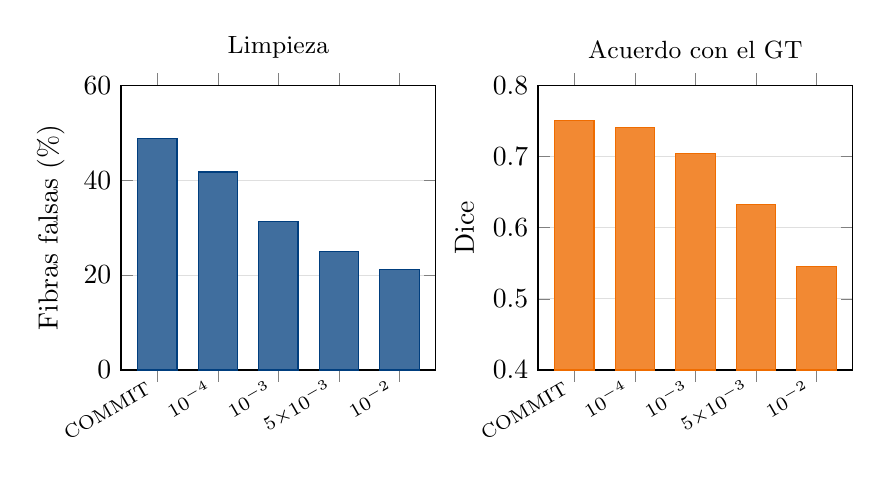
\begin{tikzpicture}
\begin{axis}[
  name=a, width=0.46\textwidth, height=5.2cm, ybar, bar width=0.5cm,
  symbolic x coords={COMMIT,{$10^{-4}$},{$10^{-3}$},{$5{\times}10^{-3}$},{$10^{-2}$}},
  xtick=data, xticklabel style={font=\scriptsize,rotate=30,anchor=east},
  ylabel={Fibras falsas (\%)}, ymin=0, ymax=60, ymajorgrids, grid style={gray!25},
  title={\small Limpieza}, enlarge x limits=0.15
]
\addplot[fill=cimatblue!75,draw=cimatblue] coordinates {(COMMIT,48.7) ({$10^{-4}$},41.7) ({$10^{-3}$},31.2) ({$5{\times}10^{-3}$},25.0) ({$10^{-2}$},21.2)};
\end{axis}
\begin{axis}[
  at={(a.east)}, anchor=west, xshift=1.3cm, width=0.46\textwidth, height=5.2cm, ybar, bar width=0.5cm,
  symbolic x coords={COMMIT,{$10^{-4}$},{$10^{-3}$},{$5{\times}10^{-3}$},{$10^{-2}$}},
  xtick=data, xticklabel style={font=\scriptsize,rotate=30,anchor=east},
  ylabel={Dice}, ymin=0.4, ymax=0.8, ymajorgrids, grid style={gray!25},
  title={\small Acuerdo con el GT}, enlarge x limits=0.15
]
\addplot[fill=warnorange!80,draw=warnorange] coordinates {(COMMIT,0.750) ({$10^{-4}$},0.740) ({$10^{-3}$},0.704) ({$5{\times}10^{-3}$},0.633) ({$10^{-2}$},0.545)};
\end{axis}
\end{tikzpicture}
\caption{Efecto de $\lambda$ en COMMIT2: al subirlo bajan las fibras falsas, pero tambi\'en
el Dice. Los valores $10^{-4}$ y $10^{-3}$ conservan los 21 haces.}
\label{fig:lambda}
\end{figure}

$\lambda$ funciona como una perilla entre limpieza y cobertura. Los valores $10^{-4}$ y
$10^{-3}$ son los \'utiles: conservan los 21 haces, con 41.7\,\% y 31.2\,\% de falsas.
Para $\lambda=10^{-2}$, nuestra corrida deja 36\,928 hilos con peso positivo, frente a
62\,779 reportados por una corrida previa del equipo con el mismo $\lambda$; la diferencia
puede venir de los pesos de grupo adaptativos, de usar 85 regiones (con el nodo 0) o de un
tractograma distinto, y no est\'a resuelta.

\subsection{Combinaci\'on de m\'etodos}

Para combinar pesos de escalas distintas se usa el promedio de percentiles
(véase Secci\'on~\ref{sec:norm}). Con solo COMMIT y SIFT2 la combinaci\'on no sirve: el umbral \'optimo es
siempre el m\'inimo (conservar casi todo), subir el umbral de 0.1 a 0.5 aumenta las falsas
de 47.1\,\% a 59.5\,\% y ninguna versi\'on supera al tractograma sin filtrar. La causa
principal es la longitud: ambos favorecen hilos cortos y la etiqueta MDF marca como falsos
casi todos los cortos (solo el 3.9\,\% de los hilos de menos de 56~mm resulta verdadero).

La mejor combinaci\'on es \textbf{COMMIT2 + LiFE}, los dos m\'etodos con AUC $>0.5$ hilo por
hilo, con percentil global (Tabla~\ref{tab:combo}). Su puntaje combinado tiene AUC 0.713, por
encima de COMMIT2 (0.684) y de LiFE (0.655) por separado; es la primera combinaci\'on en
lograrlo.

\begin{table}[H]
\centering
\small
\begin{tabularx}{\textwidth}{@{}Xrrrrrr@{}}
\toprule
\textbf{Versi\'on} & \textbf{Hilos} & \textbf{Haces} & \textbf{\% falsas} & \textbf{Cobert.} & \textbf{Dice} & \textbf{MDF (mm)}\\
\midrule
Sin filtrar        & 100\,000 & 21 & 45.2 & 0.818 & 0.750 & 2.47\\
COMMIT2 + LiFE     & 66\,287  & 21 & \textbf{33.8} & 0.756 & 0.736 & 2.59\\
\bottomrule
\end{tabularx}
\caption{Tractograma filtrado con COMMIT2 + LiFE (percentil global, $u=0.1$) frente al
tractograma sin filtrar.}
\label{tab:combo}
\end{table}

Con el mismo n\'umero de hilos conservados (Tabla~\ref{tab:mismon}), la combinaci\'on tiene
menos falsas que cualquiera de los dos m\'etodos solos en $u=0.1$ y $0.2$, a cambio de algo
menos de cobertura que COMMIT2. Desde $u=0.3$, COMMIT2 solo ya es igual o mejor.
Normalizar por rangos de longitud ayudaba cuando se combinaban COMMIT y SIFT2 (corrige su
sesgo hacia los cortos), pero aqu\'i empeora el resultado (AUC 0.65 contra 0.71), porque
COMMIT2 y LiFE favorecen los hilos largos y la longitud s\'i predice la pertenencia a un
haz.

\begin{table}[H]
\centering
\small
\begin{tabularx}{\textwidth}{@{}lXXX@{}}
\toprule
\textbf{$u$ (hilos)} & \textbf{COMMIT2 + LiFE} & \textbf{COMMIT2 solo} & \textbf{LiFE solo}\\
\midrule
0.1 (66\,287) & \textbf{33.8} / 0.756 / 0.736 & 38.1 / 0.787 / 0.747 & 37.0 / 0.748 / 0.733\\
0.2 (54\,352) & \textbf{29.9} / 0.689 / 0.702 (20) & 33.4 / 0.765 / 0.744 & 33.5 / 0.702 / 0.717\\
0.3 (42\,402) & 26.5 / 0.591 / 0.624 (19) & \textbf{26.1} / 0.707 / 0.718 (20) & 31.1 / 0.624 / 0.672 (20)\\
\bottomrule
\end{tabularx}
\caption{Mismo n\'umero de hilos conservados: \% de falsas / cobertura / Dice (entre
par\'entesis, haces detectados si son menos de 21). Percentil global.}
\label{tab:mismon}
\end{table}

\subsection{C\'alculo de la etiqueta de Hausdorff}
\label{sec:haus}

La estimaci\'on inicial era de $\approx$3 d\'ias por cada 10\,000 hilos. La fuerza bruta
compara cada hilo ($\approx$45 puntos a 2~mm) contra los $\approx$10 millones de puntos del
GT remuestreado, es decir $\approx$450 millones de distancias por hilo; medimos $\approx$22~s
por hilo, lo que extrapola a $\approx$2.5 d\'ias por 10\,000 hilos y coincide con la
estimaci\'on.

La poda se basa en una desigualdad. Si $d_H(y,g)<10$~mm, \emph{cada} punto de $y$ est\'a a
menos de 10~mm de $g$; en particular, su inicio, su punto medio y su final. Por lo tanto,
un hilo $g$ del GT sin ning\'un punto a menos de 10~mm de alguna de esas tres posiciones no
puede cumplir $d_H<10$ y se descarta sin calcular nada. En la pr\'actica se construye un
\'arbol KD con los puntos del GT remuestreado cada 2~mm, se consulta qu\'e hilos del GT pasan
cerca del inicio, del medio y del final de $y$, se intersectan las tres listas (quedan
decenas, no 189\,985) y la distancia de Hausdorff exacta se calcula solo contra esos
candidatos. Si no queda ninguno, o el mejor supera 10~mm, el hilo se marca como
``a m\'as de 10~mm''.

\begin{table}[H]
\centering
\small
\begin{tabular}{@{}lrr@{}}
\toprule
 & \textbf{Fuerza bruta} & \textbf{Con poda}\\
\midrule
Tiempo por hilo        & $\approx$22~s       & $\approx$0.12~s\\
10\,000 hilos          & $\approx$2.5 d\'ias & $\approx$20~min\\
100\,000 hilos         & $\approx$25 d\'ias  & $\approx$3.3~h en una computadora;\\
                       &                     & $\approx$35~min por bloque con 7\\
\bottomrule
\end{tabular}
\caption{Costo del c\'alculo de la etiqueta de Hausdorff.}
\label{tab:haus}
\end{table}

\textbf{Verificaci\'on.} En 40 hilos al azar contra los 189\,985 del GT, 23 de 40 tuvieron
correspondencia a menos de 10~mm tanto con fuerza bruta como con la poda, los mismos 40
hilos quedaron igual clasificados, y la diferencia m\'axima entre ambos m\'etodos con el mismo
remuestreo fue 0.0~mm: la poda no pierde ning\'un candidato. El remuestreo a 2~mm, en
comparaci\'on con 1~mm, cambi\'o la distancia en promedio 0.032~mm y a lo m\'as 0.236~mm, muy por
debajo de los $\eps_H$ considerados (2--10~mm). 


\textbf{Limitaciones:} el resultado solo
distingue ``$<10$~mm'' de ``m\'as''; la muestra de validaci\'on es de 40 hilos (la fuerza bruta
completa es justo lo que se quiere evitar); y el error de remuestreo se midi\'o contra 1~mm,
no contra el c\'alculo continuo. En una prueba con 300 hilos, el 58\,\% tuvo un hilo del GT a
menos de 10~mm. El c\'alculo completo se reparte en 7 bloques de $\approx$14\,286 hilos entre
distintas computadoras; los resultados son independientes entre hilos, as\'i que repartir no
cambia nada.

% =================== 5. DISCUSIÓN ===================
\section{Discusión}

En este trabajo se parti\'o de un \'unico tractograma de 100\,000 hilos y se pes\'o con los m\'etodos SIFT2, LiFE, COMMIT y COMMIT2, respetando en los cuatro el mismo orden de hilos. Con esos vectores se compararon los m\'etodos entre s\'i y contra el GT a nivel de conexi\'on y a nivel de hilo, se barri\'o el par\'ametro $\lambda$ de COMMIT2 (Tabla~\ref{tab:lambda}), se ensay\'o la combinaci\'on por percentiles (Tabla~\ref{tab:combo}) y se dej\'o lista y validada la etiqueta por Hausdorff.

Al obtener la matriz de conectividad de cada método, COMMIT y SIFT2 alcanzan un AUC por conexi\'on de $0.829$ y $0.850$ (ir Tabla~\ref{tab:matrices}) y, al mismo tiempo, ordenan al rev\'es a los hilos individuales (ir Figura~\ref{fig:auc}). Sus pesos sirven para estimar la fuerza de una conexi\'on, no para elegir hilos. LiFE es el \'unico que funciona en los dos niveles, con la \'unica matriz ponderada que supera al conteo y un AUC por hilo de $0.655$.

%\textbf{Matriz y hilo cuentan historias distintas.} Una matriz solo dice qu\'e regiones se conectan; no importa si un hilo concreto es correcto. Por eso COMMIT y SIFT2 alcanzan AUC 0.83--0.85 por conexi\'on y, al mismo tiempo, ordenan al rev\'es a los hilos individuales. Sus pesos sirven para estimar la fuerza de una conexi\'on, no para elegir hilos.

Se propuso una cuarta variable (longitud) en una versión aparte del modelo para medir cu\'anto aporta cada m\'etodo adem\'as de ella. A nivel de conexi\'on, la correlaci\'on de COMMIT con el GT sube de $0.731$ a $0.881$ cuando su peso se multiplica por la longitud del hilo (Tabla~\ref{tab:matrices}), ya que est\'a definido por unidad de longitud. Hilo por hilo, los verdaderos miden $107.5$~mm de media y los falsos $73.6$~mm, de modo que la longitud sola alcanza un AUC de $0.747$ y supera a los cuatro m\'etodos (Figura~\ref{fig:auc}). Dentro de un mismo tramo de longitud, COMMIT y SIFT2 caen a valores de entre $0.45$ y $0.57$.

%\textbf{La longitud domina.} Es el hallazgo m\'as robusto: aparece en los pesos de COMMIT (por construcci\'on, al ser por unidad de longitud), en la etiqueta MDF y en la comparaci\'on por hilo, donde la longitud sola le gana a los cuatro m\'etodos (0.747). Cualquier filtro o modelo que no la considere puede aparentar un desempe\~no que en realidad viene de ella. Por eso se propone incluir la longitud como una cuarta variable en una versi\'on aparte del modelo, para medir cu\'anto aporta cada m\'etodo adem\'as de ella.

La mejor combinaci\'on encontrada, COMMIT2 + LiFE con percentil global, baja las fibras falsas de $45.2$\,\% a $33.8$\,\% y conserva los $21$ haces (Tabla~\ref{tab:combo}). El margen es estrecho, porque a partir de $u=0.3$ COMMIT2 por s\'i solo iguala o supera a la combinaci\'on con el mismo n\'umero de hilos (Tabla~\ref{tab:mismon}). Combinar ayuda solo
cuando los m\'etodos que entran aportan informaci\'on por hilo, y por eso a\~nadir COMMIT y SIFT2 al promedio empeora el puntaje.

Ahora bien, el orden en que quedan los m\'etodos hilo por hilo depende de la etiqueta que se use para decidir si un hilo es verdadero. La etiqueta MDF, con un umbral de $5$~mm, marca como verdadero al $54.8$\,\% de los hilos, pero solo al $3.9$\,\% de los menores de $56$~mm. Por lo que, se castigan a los hilos cortos. De aquí que, el COMMIT proviene de la etiqueta y no del m\'etodo (Figura~\ref{fig:auc}). La versi\'on dirigida de
Hausdorff pregunta si el hilo est\'a \emph{dentro} de un haz y no castiga a los cortos que s\'i caen en uno, as\'i que
puede cambiar el orden de los m\'etodos. Como se conoce c\'omo difieren las dos en
teor\'ia pero no cu\'anto en estos datos, conviene reportar ambas.

%\textbf{La etiqueta condiciona la conclusi\'on.} La MDF~$<5$~mm marca como verdadero al 54.8\,\% de los hilos, pero solo al 3.9\,\% de los menores de 56~mm; una etiqueta por m\'ascara, en cambio, marca al 94\,\%. Ninguna es adecuada, y parte de ``COMMIT va al rev\'es'' proviene de la etiqueta. La de Hausdorff dirigida, que pregunta si el hilo est\'a \emph{dentro} de un haz, no castiga a los hilos cortos que s\'i caen en uno, y por ello puede cambiar el orden de los m\'etodos. Dado que se conoce c\'omo difieren en teor\'ia pero no cu\'anto en estos datos, conviene reportar ambas.

Cabe señalar que, del análisis anterior hay diferentes limitaciones. (i) El Dice no sirve para elegir el umbral: queda entre $0.746$ y $0.759$ en $40$ combinaciones y el m\'aximo es siempre ``sin filtrar''. (ii) El umbral se elige con el mismo GT con que se eval\'ua, lo que es optimista. (iii) Eliminar el peso $0$ es solo una hip\'otesis; sin embargo, SIFT2 nunca da $0$, por lo que se requiere un corte arbitrario. (iv) COMMIT2 solo tiene $36\,928$ hilos con peso positivo, y al compararlo con el mismo $n$ mayor se completa con ceros al azar. (v) La AUC por extremos de COMMIT2 ($0.80$) est\'a inflada porque sus grupos se definen con los mismos pares de regiones que esa etiqueta.

% =================== 6. ESTADO ===================
\section{Estado del trabajo y siguientes pasos}
\label{sec:estado}

\begin{table}[H]
\centering
\small
\begin{tabularx}{\textwidth}{@{}lXl@{}}
\toprule
\textbf{Paso} & \textbf{Descripci\'on} & \textbf{Estado}\\
\midrule
A & Vector de 100\,000 pesos por m\'etodo (SIFT2, LiFE, COMMIT; COMMIT2 como extra) & Hecho\\
B & Normalizar a $(0,1)$, filtrar con $\eps$ y comparar cada m\'etodo con el GT & Parcial\\
C & Etiqueta 0/1 por hilo con Hausdorff & En curso\\
D & Modelo $(x_S,x_L,x_C)\to$ etiqueta y su tractograma filtrado & Pendiente\\
\bottomrule
\end{tabularx}
\caption{Estado frente al objetivo.}
\label{tab:estado}
\end{table}

\textbf{Paso B.} Existe el filtrado con un $\eps$ dado (normalizando por el m\'aximo), pero
falta el barrido de $\eps$ (por ejemplo, de 0.01 a 0.9) con comparaci\'on a igual n\'umero de
hilos conservados, y decidir entre normalizaci\'on por m\'inimo--m\'aximo o por percentil.

\textbf{Paso C.} El script est\'a probado; falta ejecutarlo en las 7 computadoras y unir los
bloques. Se propone $\eps_H=5$~mm ($\approx$2.5 v\'oxeles de 2~mm, igual al valor de la MDF
para poder comparar) y barrer 2, 3, 5, 7 y 10~mm. Despu\'es se compara con la etiqueta MDF
(matriz de confusi\'on para varios $\eps$) y se revisa si cambia el orden de los m\'etodos.

\textbf{Paso D.} Se propone una regresi\'on log\'istica
\begin{equation}
  \Pr(y_i=1)=\sigma\big(\alpha\,x_{iS}+\beta\,x_{iL}+\gamma\,x_{iC}+b\big),
\end{equation}
con el voto (v\'alido si al menos 2 de 3 m\'etodos lo aceptan) y el filtro simple por $\eps$
como comparaciones. Debe separarse entrenamiento y prueba (por ejemplo, con distintos
bloques de hilos o validaci\'on cruzada) y reportar solo sobre la parte de prueba. Antes de
interpretar el modelo hay que comprobar con Hausdorff el sentido en que ordenan COMMIT y
SIFT2.

\textbf{Otros pendientes:} una etiqueta intermedia por haz (por ejemplo, la fracci\'on de
puntos del hilo a $\le2$~mm de un haz), elegir el umbral con la mitad de los haces y evaluar
con la otra mitad, decidir $\lambda$ en COMMIT2, y aislar el efecto de la correcci\'on del
eje $y$ en COMMIT y LiFE.

% =================== 7. CONCLUSIONES ===================
\section{Conclusiones}

Con un tractograma compartido de 100\,000 hilos se obtuvieron y compararon tres vectores de
pesos (y COMMIT2) contra el GT. A nivel de matriz, LiFE es el \'unico que mejora al conteo;
COMMIT mejora al multiplicarlo por la longitud. A nivel de hilo, COMMIT y SIFT2 ordenan al
rev\'es de lo esperado con la etiqueta MDF, y COMMIT2 y LiFE s\'i separan; la longitud sola
supera a todos, por lo que cualquier modelo debe considerarla expl\'icitamente. La mejor
combinaci\'on actual es COMMIT2 + LiFE, que reduce las fibras falsas de 45.2\,\% a 33.8\,\%
sin perder haces, aunque con $u\ge0.3$ COMMIT2 solo es igual o mejor. Adem\'as, la poda
espacial hace viable la etiqueta de Hausdorff (de d\'ias a $\approx$35 minutos por bloque) con
resultado id\'entico a la fuerza bruta en la muestra verificada. Los resultados dependen de
la etiqueta y se midieron con la MDF; su confirmaci\'on con Hausdorff y el entrenamiento del
modelo son los pasos que faltan para cerrar el objetivo.

% =================== APÉNDICE ===================
\appendix
\section{Reproducibilidad}
\label{app:repro}

El entorno se crea con \code{conda env create -f environment.yml} (MRtrix 3.0.8, Python
3.13, COMMIT 2.4.2, AMICO 2.1.1) o con un \textit{venv} y \code{requirements.txt} (macOS, con
MRtrix3 3.0.8 aparte). COMMIT falla con rutas que tengan acentos o espacios.

\begin{table}[H]
\centering
\small
\begin{tabularx}{\textwidth}{@{}lXl@{}}
\toprule
\textbf{Script} & \textbf{Qu\'e hace} & \textbf{Objetivo}\\
\midrule
\code{01\_preprocess.sh}    & gradientes con $y$ invertido, m\'ascara, respuesta y FOD & base\\
\code{02\_tractography.sh}  & tractograma, longitudes y pesos SIFT2 & A\\
\code{03\_commit.sh}        & pesos COMMIT & A\\
\code{05\_life.sh}          & pesos LiFE (entregados por el equipo de LiFE) & A\\
\code{04\_matrices.sh}      & matrices $84\times84$ y su evaluaci\'on & extra\\
\code{06\_commit2.sh}       & COMMIT2 y su matriz & extra\\
\code{07\_normalizacion.sh} & normalizaci\'on por percentil y combinaci\'on & B (parcial)\\
\code{08\_hausdorff.sh}     & etiqueta de Hausdorff por bloques & C\\
\code{09\_filtrar\_pesos.sh}& normalizar por el m\'aximo y filtrar con $\eps$ & B\\
\bottomrule
\end{tabularx}
\caption{Scripts del repositorio y qu\'e producen.}
\label{tab:scripts}
\end{table}

\textbf{N\'umeros de control} para verificar una reproducci\'on: \code{tckstats} del
tractograma da media 92.13, mediana 95.21 y 100\,000 hilos; COMMIT conserva los 100\,000
hilos, con NRMSE $0.106\pm0.039$ y 44\,780 pesos en cero (45\,\%); y la matriz del GT tiene
529 conexiones. Si se olvida invertir $y$, se nota: hilos de $\approx$42~mm de media y solo
$\approx$21\,\% de conexiones reales en la matriz.

% =================== REFERENCIAS ===================
\begin{thebibliography}{99}
\small
\bibitem{maierhein2017} K.~H. Maier-Hein \textit{et al.} The challenge of mapping the human
  connectome based on diffusion tractography. \textit{Nature Communications}, 8:1349, 2017.
\bibitem{smith2015} R.~E. Smith, J.-D. Tournier, F. Calamante, A. Connelly. SIFT2: Enabling
  dense quantitative assessment of brain white matter connectivity using streamlines
  tractography. \textit{NeuroImage}, 119:338--351, 2015.
\bibitem{pestilli2014} F. Pestilli, J.~D. Yeatman, A. Rokem, K.~N. Kay, B.~A. Wandell.
  Evaluation and statistical inference for human connectomes. \textit{Nature Methods},
  11:1058--1063, 2014.
\bibitem{daducci2015} A. Daducci, A. Dal~Pal\`u, A. Lemkaddem, J.-P. Thiran. COMMIT: Convex
  optimization modeling for microstructure informed tractography. \textit{IEEE Transactions
  on Medical Imaging}, 34(1):246--257, 2015.
\bibitem{daducci2015amico} A. Daducci, E.~J. Canales-Rodr\'iguez, H. Zhang, T.~B. Dyrby,
  D.~C. Alexander, J.-P. Thiran. Accelerated Microstructure Imaging via Convex Optimization
  (AMICO) from diffusion MRI data. \textit{NeuroImage}, 105:32--44, 2015.
\bibitem{schiavi2020} S. Schiavi \textit{et al.} A new method for accurate in vivo mapping
  of human brain connections using microstructural and anatomical information.
  \textit{Science Advances}, 6(31):eaba8245, 2020.
\bibitem{tournier2019} J.-D. Tournier \textit{et al.} MRtrix3: A fast, flexible and open
  software framework for medical image processing and visualisation. \textit{NeuroImage},
  202:116137, 2019.
\bibitem{tournier2007} J.-D. Tournier, F. Calamante, A. Connelly. Robust determination of the
  fibre orientation distribution in diffusion MRI: non-negativity constrained super-resolved
  spherical deconvolution. \textit{NeuroImage}, 35(4):1459--1472, 2007.
\bibitem{tournier2010} J.-D. Tournier, F. Calamante, A. Connelly. Improved probabilistic
  streamlines tractography by 2nd order integration over fibre orientation distributions.
  \textit{Proc. ISMRM}, 18:1670, 2010.
\bibitem{garyfallidis2014} E. Garyfallidis \textit{et al.} Dipy, a library for the analysis of
  diffusion MRI data. \textit{Frontiers in Neuroinformatics}, 8:8, 2014.
\bibitem{garyfallidis2012} E. Garyfallidis, M. Brett, M.~M. Correia, G.~B. Williams,
  I. Nimmo-Smith. QuickBundles, a method for tractography simplification. \textit{Frontiers
  in Neuroscience}, 6:175, 2012.
\bibitem{panagiotaki2012} E. Panagiotaki \textit{et al.} Compartment models of the diffusion
  MR signal in brain white matter: A taxonomic comparison. \textit{NeuroImage},
  59(3):2241--2254, 2012.
\end{thebibliography}

\end{document}
